\chapter{Systembeskrivelse}
\vspace{-1cm}
På Ingeniørhøjskolen Aarhus Universitet forefindes en AeroQuad ARF Quadrocopter. 
Målet med projektet er at omdanne quadrocopteren til en autonom overvågningsdrone.

Dronen skal ud fra brugers anvisninger overvåge og tage billeder af et defineret område. 
Dronen tilgås via en webapplikation der fungerer som en grafisk brugerflade mellem bruger og systemet.  Via webapplikationen kan bruger oprette flyveopsætninger til drone samt se billeder og flyverute fra tidligere flyvninger.  
Når der laves ny flyveopsætning vælger bruger en række GPS positioner som dronen skal flyve til, flyvehøjde og hvorvidt der skal tages billeder ved de valgte GPS positioner. Når bruger har lavet en ny flyveopsætning, stilles flyveopsætningen tilgængelig for dronen på server.  

Da dronen skal flyve autonomt, er det vigtigt at den kan orientere sig på egen hånd. Derfor er dronen udstyret med GPS, afstandssensorer og kompas.
Til enhver tid skal kommunikation mellem drone og server foregå via mobilt netværk. Der gøres hovedsageligt brug af 3G netværket, men i områder med dårlig forbindelse vil der blive gjort brug af 2G som fall-back netværk. 

\vspace{-0.5cm}

\section*{Systemskitse}
\vspace{-0.5cm}
Bruger benytter en computer til at tilgå webapplikation og lave en ny flyveopsætning. Når bruger har lavet en ny flyveopsætning, overføres flyveopsætningen via Internettet til server, hvor den gøres tilgængelig for dronen.
 
Via det mobile 3G netværk kommunikerer drone med server. 
Inden flyvning påbegyndes henter drone flyveopsætning fra server og under flyvning sender dronen information om nuværende GPS position og overfører billeder til server. 
Under flyvning kontrollerer drone løbende egen GPS position via kommunikation med GPS satellitter. Dette gør den for at opdatere egen position og for efterfølgende at kunne beregne den korrekte flyveorientering. 



\vspace{-5pt}
%Systemskitse
\begin{figure}[H]
\centering
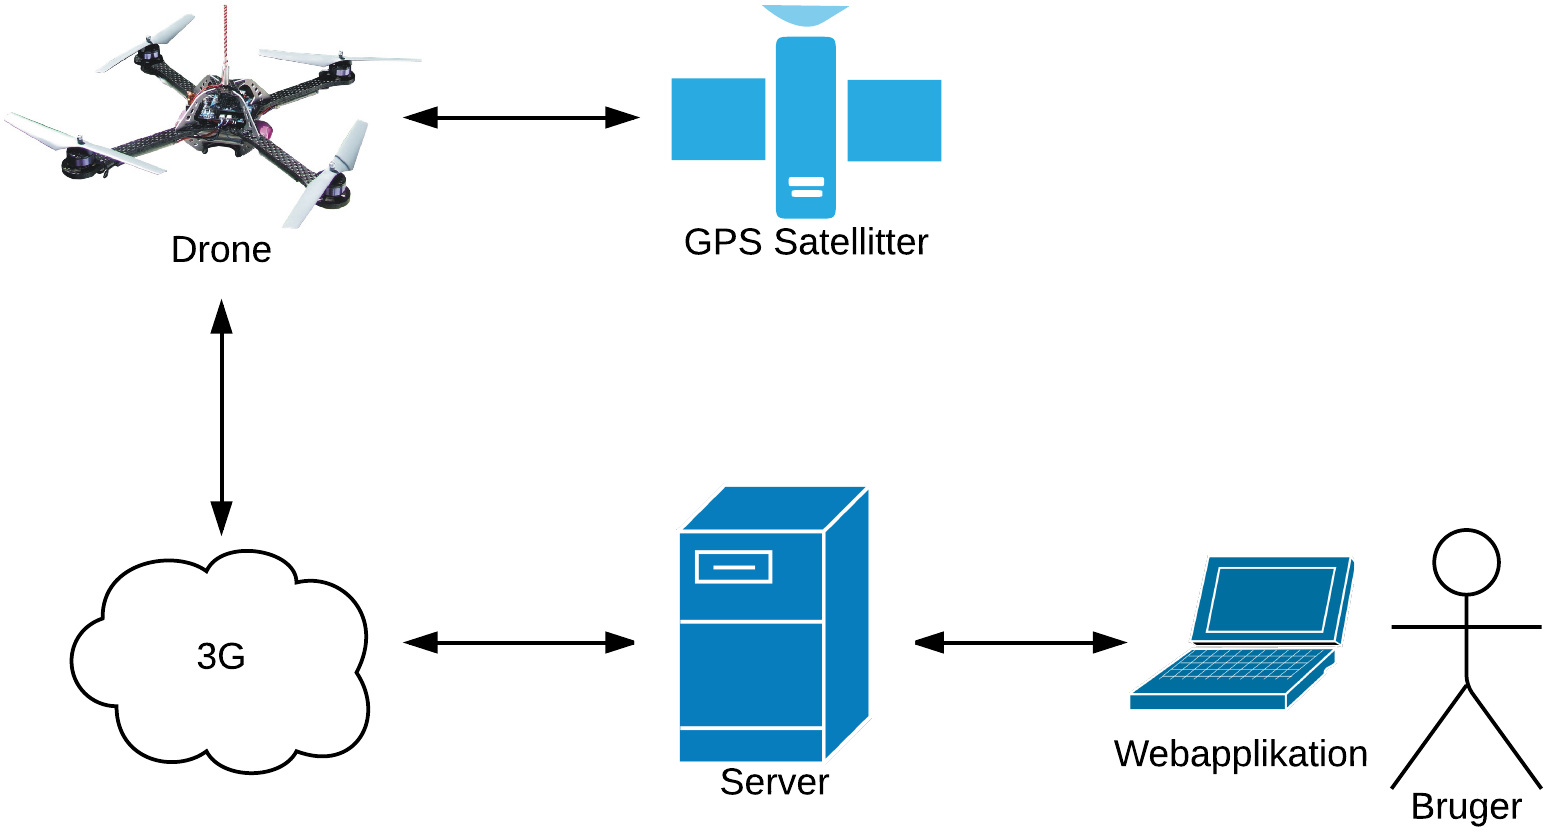
\includegraphics[width=0.8\textwidth]{Billeder/Projektbeskrivelse.png}
\vspace{-.3cm}
\caption{Systemskitse}
\label{fig:Systemskitse}
\end{figure}